\documentclass[a4paper,10pt]{article}
\usepackage{graphicx}
\usepackage{amsmath}
\usepackage{amssymb}
\usepackage[italian]{babel}
\usepackage[T1]{fontenc}
\usepackage[utf8]{inputenc}
\usepackage[margin=0.42in]{geometry}
\usepackage{caption}
\usepackage{subcaption}

\begin{document}
\pagenumbering{gobble}
\begin{center}
\Large
\noindent
\textbf{Homework 2}\\
\normalsize
Strumenti per la valutazione delle prestazioni di rete\\
\end{center}
\noindent
\textbf{Comando \texttt{ping}}\\
Il primo comando di cui è stato studiato il comportamento è stato il comando \texttt{ping}. Grazie a questo software è stato possibile, mediante l'utilizzo di un'apposita opzione da linea di comando (\texttt{-t}) misurare sperimentalmente il numero di \textit{hop} che separano la macchina client dal server. La misura è stata effettuata incrementando gradualmente il campo TTL dell'header IP e verificando per quale valore del campo i pacchetti cominciavano ad arrivare a destinazione senza essere scartati prima. Il numero di hop è stato in questo modo misurato essere pari a \textbf{13}.\\

\noindent
Lo stesso comando è stato utilizzato, con l'aggiunta di ulteriori opzioni (\texttt{-s} e \texttt{-c}), al fine di misurare il RTT minimo, medio e massimo tra client e server. I risultati sono stati rappresentati graficamente e sono riportati in Figura \ref{fig:rttfig}.

\begin{figure}[h!]
     \centering
     \begin{subfigure}[b]{0.325\textwidth}
         \centering
         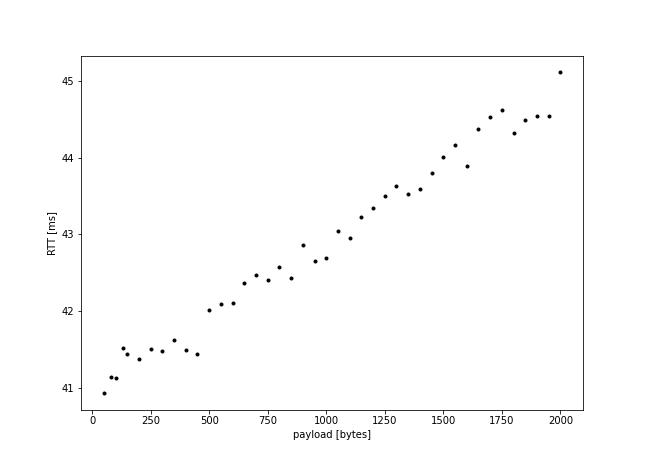
\includegraphics[width=\textwidth]{img/min.png}
         \caption{RTT minimo.}
         \label{fig:rttmin}
     \end{subfigure}
     \hfill
     \begin{subfigure}[b]{0.325\textwidth}
         \centering
         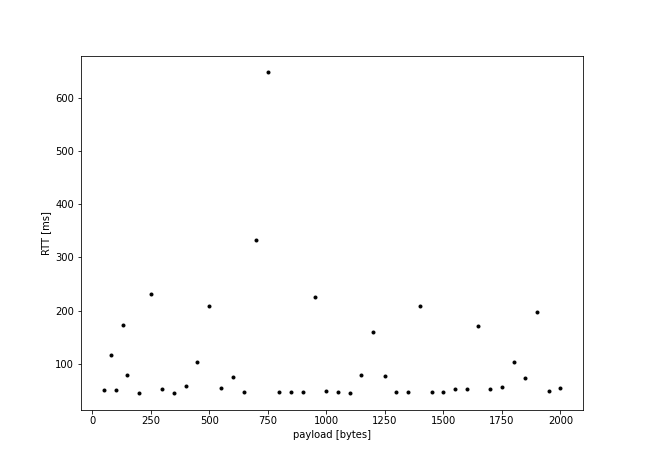
\includegraphics[width=\textwidth]{img/max.png}
         \caption{RTT massimo.}
         \label{fig:rttmax}
     \end{subfigure}
     \hfill
     \begin{subfigure}[b]{0.325\textwidth}
         \centering
         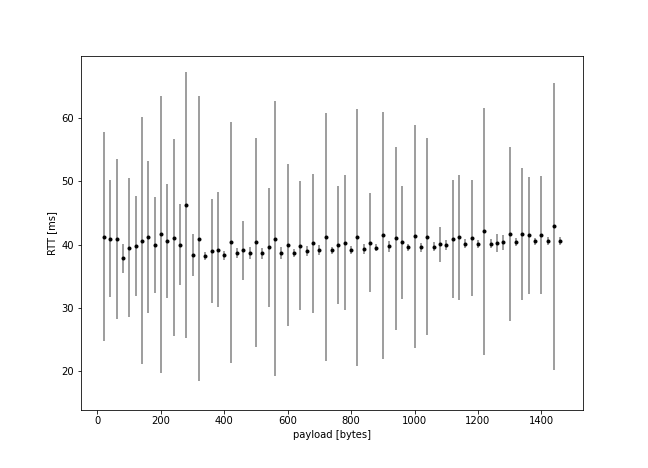
\includegraphics[width=\textwidth]{img/avg.png}
         \caption{RTT medio e std.}
         \label{fig:rttavg}
     \end{subfigure}
        \caption{Andamento del RTT al variare della dimensione del payload.}
        \label{fig:rttfig}
\end{figure}
\noindent
Ai dati relativi al RTT minimo è stata applicata la regressione lineare, in modo tale da poterne successivamente ricavare l'intercetta $q$ (corrispondente al tempo di propagazione del segnale) e il coefficiente angolare $m$. Quest'ultimo è infatti legato al valore del bitrate mediante l'equazione 
\vspace{-0.3cm}
\begin{align}
m = 2 \cdot \sum_{i=1}^{n}  \frac{1}{R_i} \approx \frac{2}{min_i R_i}
\label{eq:ris}
\end{align}
Il bitrate calcolato invertendo l'Equazione (\ref{eq:ris}) è risultato essere pari a \textbf{6.71 Mbps}. Al fine di verifica, la regressione è stata applicata anche ai dati sul RTT medio. Inizialmente è stato considerato l'insieme completo delle misurazioni, ottenendo però un coefficiente angolare calcolato molto diverso rispetto al valore precedente. Si è quindi svolta un'operazione di \textit{data cleaning} sul dataset, in cui sono stati rimossi tutti i campioni dalla deviazione standard troppo elevata ($>10\,ms$) o appartenenti alle prime misurazioni (che si è notato essere molto meno precise rispetto alle altre), con risultati in questo caso molto simili a quelli ottenuti dai dati sul RTT minimo (stesso coefficiente angolare della retta ma diversa intercetta, la cui differenza con l'intercetta del RTT minimo potrebbe essere interpretata come \textit{ritardo medio causato dal buffering}). Una rappresentazione grafica dei risultati ottenuti in queste elaborazioni può essere ricavata dal grafico in Figura \ref{fig:regr}. 
\begin{figure}[!htb]
	\centering
	\begin{minipage}{0.33\textwidth}
     \centering
         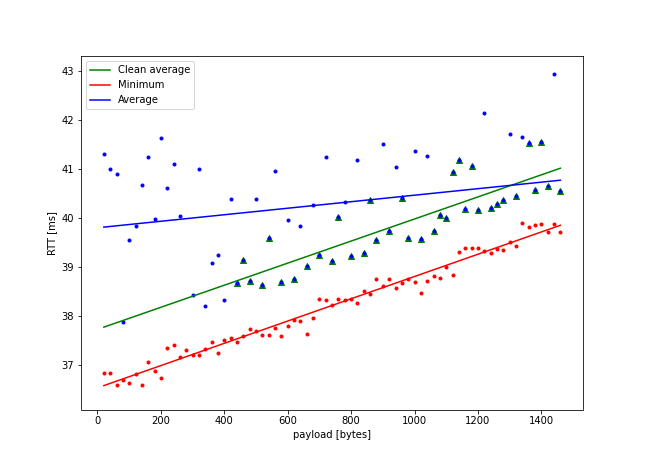
\includegraphics[width=1\linewidth]{img/clean.png}
         \caption{Regressioni lineari.}
         \label{fig:regr}
    \end{minipage}
   \begin{minipage}{0.33\textwidth}
     \centering
         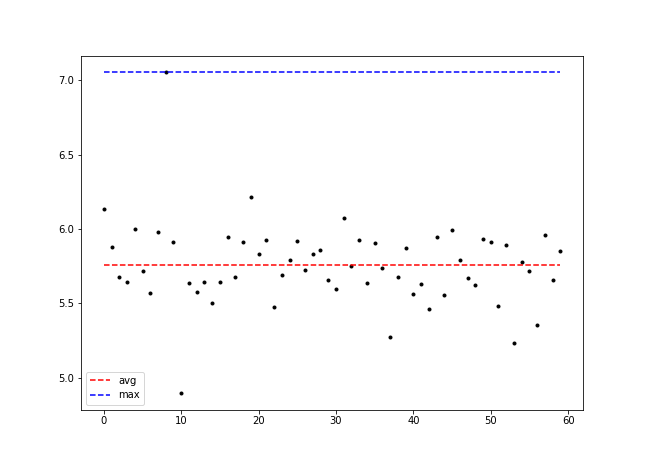
\includegraphics[width=1\linewidth]{img/iperf.png}
         \caption{Bitrate \texttt{iperf}.}
         \label{fig:iperf}
   \end{minipage}\hfill
\end{figure}

\noindent
\textbf{Comando \texttt{iperf}}\\
Il secondo comando di cui è stato studiato il comportamento è stato \texttt{iperf}, applicativo che ci ha permesso di misurare direttamente il bitrate della connessione. Anche in questo caso sono state effettuate diverse misure ad intervalli regolari, di cui è stata successivamente fatta una media (Figura \ref{fig:iperf}). Il bitrate medio così calcolato è risultato essere pari a \textbf{6.44 Mbps}.  \\

\noindent
\textbf{Conclusioni}\\
Le stime del bitrate ottenute mediante i due comandi \texttt{ping} e \texttt{iperf} sono tra loro molto simili e denotano una differenza reciproca inferiore al $5\%$, legata verosimilmente alle approssimazioni fatte nel calcolo della pendenza per i valori di bitrate del \texttt{ping} e agli errori casuali legati alla forte variabilità dello stato della rete. I risultati ottenuti si sono inoltre dimostrati realistici rispetto al collegamento Internet di cui disponeva la macchina client. In conclusione, entrambi gli strumenti utilizzati hanno ottenuto risultati tra loro coerenti.

\end{document}